\section{Programming IDEs}
There are a few specific IDEs which you may find useful in this course. Specifically, they are CLion and PyCharm, both of which are created by JetBrains. You can get access to licences for JetBrains IDEs by signing up for the \href{https://education.github.com/pack}{Github Education Pack}.

\subsection{Visual Studio Code}
Visual Studio Code is a powerful IDE that can be configured to run various programming languages. It has an array of plugins from C\/C++ to Latex, as well as Python and Raspberry Pi Plug-ins. You can learn more about Visual Studio Code \href{https://code.visualstudio.com/}{here}.

\begin{figure}[H]
\centering
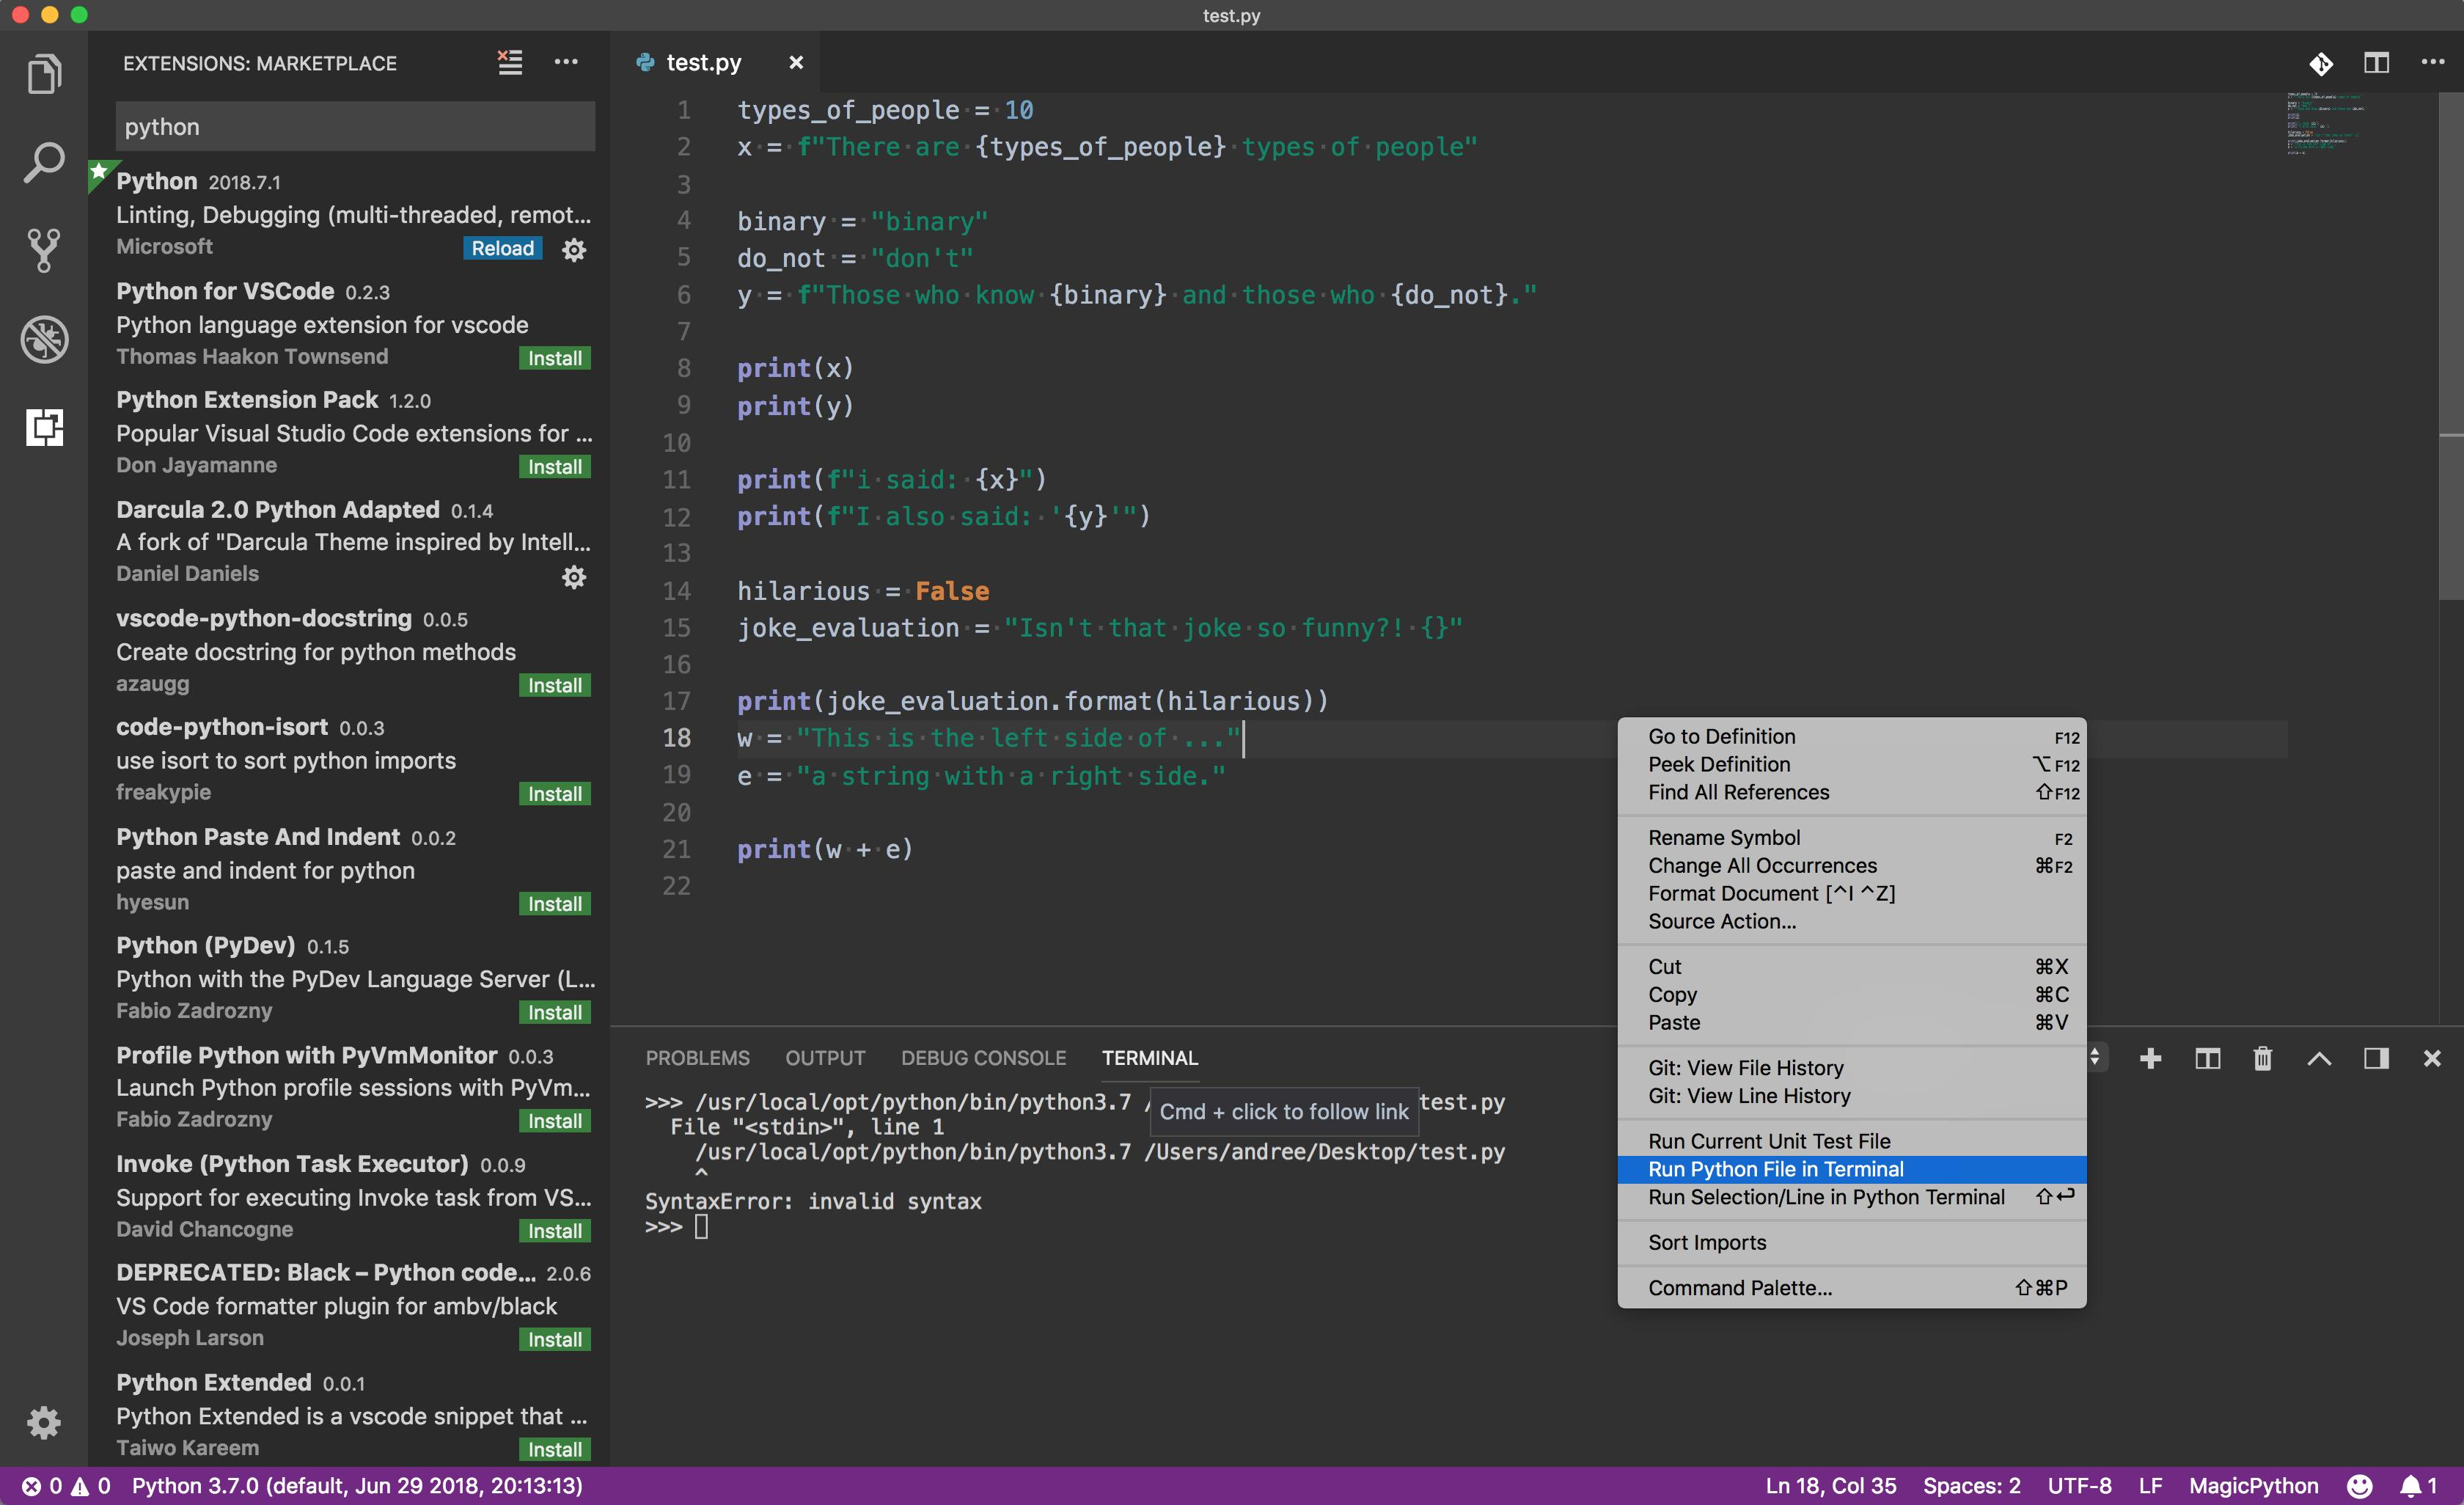
\includegraphics[width=0.8\columnwidth]{Figures/VSCode}
\caption{VSCode configured for Python \href{https://stackoverflow.com/questions/51540391/invalid-syntax-error-when-running-python-from-inside-visual-studio-code}{(image source)}}
\label{fig:VSCode}
\end{figure}


\subsection{PyCharm}
PyCharm is the Python Editor created by JetBrains. You can read more about PyCharm \href{https://www.jetbrains.com/help/pycharm/meet-pycharm.html}{here}.
Learn about setting up a virtual environment (good practice in Python) \href{https://www.jetbrains.com/help/pycharm/configuring-python-interpreter.html}{here}.

\begin{figure}[H]
\centering
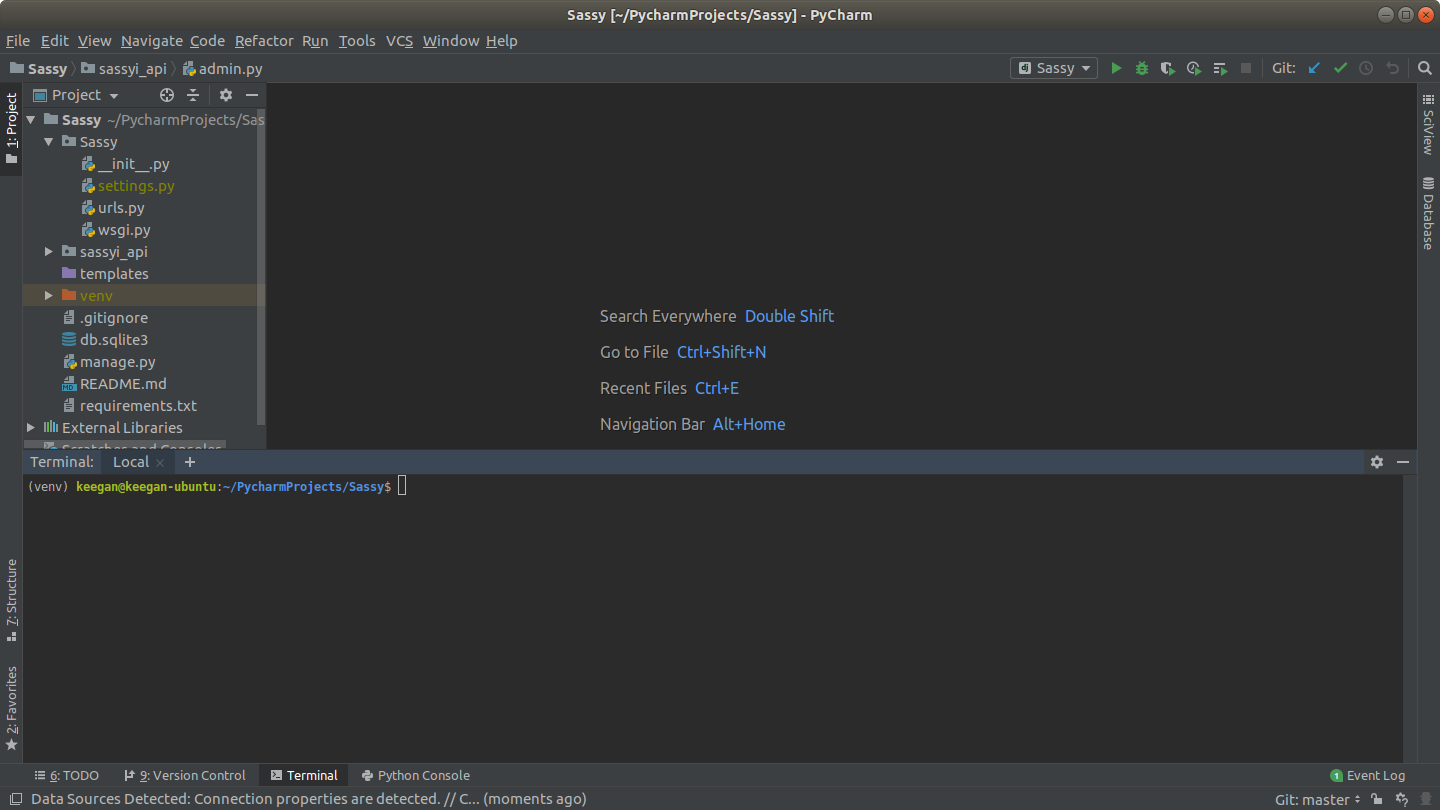
\includegraphics[width=0.8\columnwidth]{Figures/Pycharm}
\caption{The PyCharm IDE}
\label{fig:Pycharm}
\end{figure}


\subsection{CLion}
\label{sec:CLion}
CLion is a cross compilation tool developed by JetBrains that will be used in this course. 

This section covers installation and configuration of JetBrains CLion on Windows and Ubuntu. It assumes you have a JetBrains Education account (possible through the \href{https://education.github.com/pack}{Student GitHub Pack} - \href{https://education.github.com/pack}{https://education.github.com/pack}).

\subsubsection{CLion on Windows}
CLion on Windows for cross compilation requires use of the Ubuntu subsystem. At this point, it's likely better to dual boot the two operating systems. However, if you're unable to do this, you can follow through the guide below. A reminder, you don't need to use CLion - comiplation on Windows is available as pointed out in Section \ref{sec:crosscompile}.

In this guide, we're going to be working with Ubuntu 18.04 as the distribution. To install WSL, follow \href{https://docs.microsoft.com/en-us/windows/wsl/install-win10}{this tutorial}. Be sure to select Ubuntu 18.04 as your distribution.

Once you've installed it, you can start the instance by pressing the start button and searching for "Ubuntu". Upon first run, you will be asked to create a username and password. Remember these details, as they will be used later. Once you have created your username and password, run the following commands:
\begin{lstlisting}
$ sudo apt-get update 
$ sudo apt-get ugrade
$ sudo apt-get install libc6-armel-cross libc6-dev-armel-cross 
$ sudo apt-get install binutils-arm-linux-gnueabi libncurses5-dev lib32z1
$ sudo apt-get install gcc-arm-linux-gnueabi g++-arm-linux-gnueabi
\end{lstlisting}

Then, configure ssh and relevant/related items using the JetBrains script. Still on the Ubuntu sub-system, run:
\begin{lstlisting}
$ wget https://raw.githubusercontent.com/JetBrains/clion-wsl/master/ubuntu_setup_env.sh
$ bash ubuntu_setup_env.sh
\end{lstlisting}

This script configures an SSH connection on port 2222. Test is by running the following on the Ubuntu Subsystem
\begin{lstlisting}
$ ssh username@127.0.0.1 -p 2222
\end{lstlisting}

Now, open CLion. Navigate to File - Settings - Build, Execution, Deployment - Toolchains. Under environment, Select "WSL". Click the gear next to Credentials, and enter in your username and password, ensuring that the correct port number (2222) is used. You will need to change C Compiler and C++ Compilers to use the Raspberry Pi Compilers we installed in the earlier steps. Change the C compiler to use "/usr/bin/arm-linux-gnueabi-gcc" and the C++ Compiler to use "/usr/bin/arm-linux-gnueabi-g++". The configuration should now look as follows:
\begin{figure}[H]
\centering
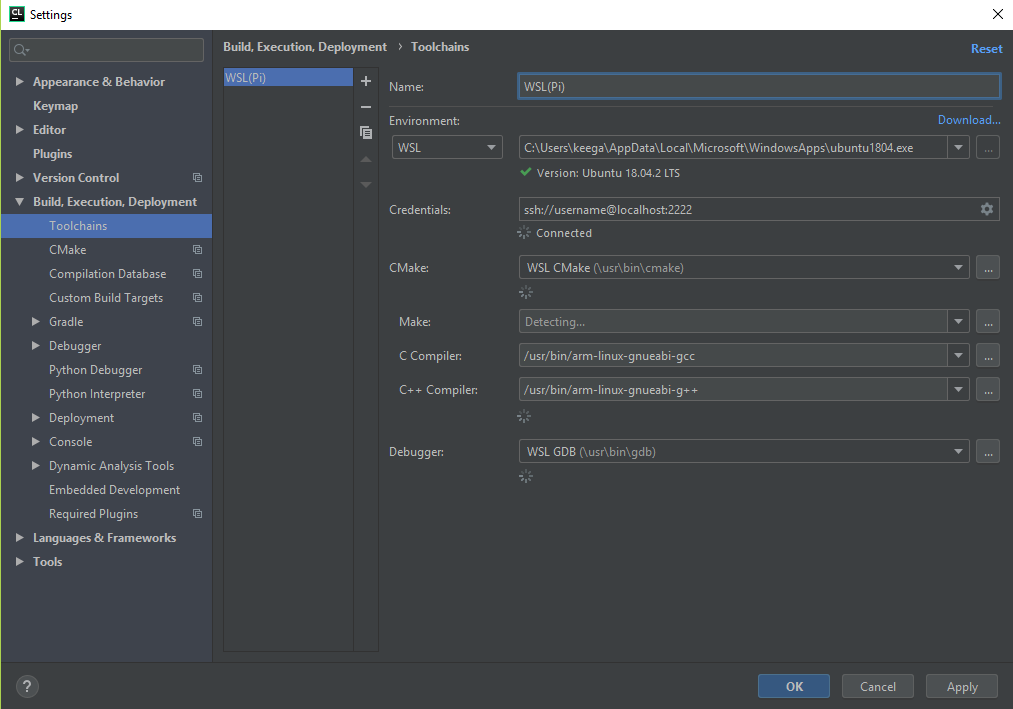
\includegraphics[width=0.8\columnwidth]{Figures/WSLConfig}
\caption{CLion WSL Configuration on Windows}
\label{fig:WSLConfig}
\end{figure}

Once you create and compile a project, you should be able to move it to the Pi using SCP (or PSCP if SCP is disabled), adding the executable flag, and running it. Do not be surprised if there is an error once you've built it on the Pi 

\subsubsection{CLion on Ubuntu}
CLion on Ubuntu is considerably easier to configure. 
Install CLion by running
\begin{lstlisting}
$ snap install clion --classic
\end{lstlisting}
RUn the following commands to install required packages:
\begin{lstlisting}
$ sudo apt-get update 
$ sudo apt-get ugrade
$ sudo apt-get install libc6-armel-cross libc6-dev-armel-cross 
$ sudo apt-get install binutils-arm-linux-gnueabi libncurses5-dev lib32z1
$ sudo apt-get install gcc-arm-linux-gnueabi g++-arm-linux-gnueabi
\end{lstlisting}

Your configuration file should be as follows:
\begin{figure}[H]
\centering
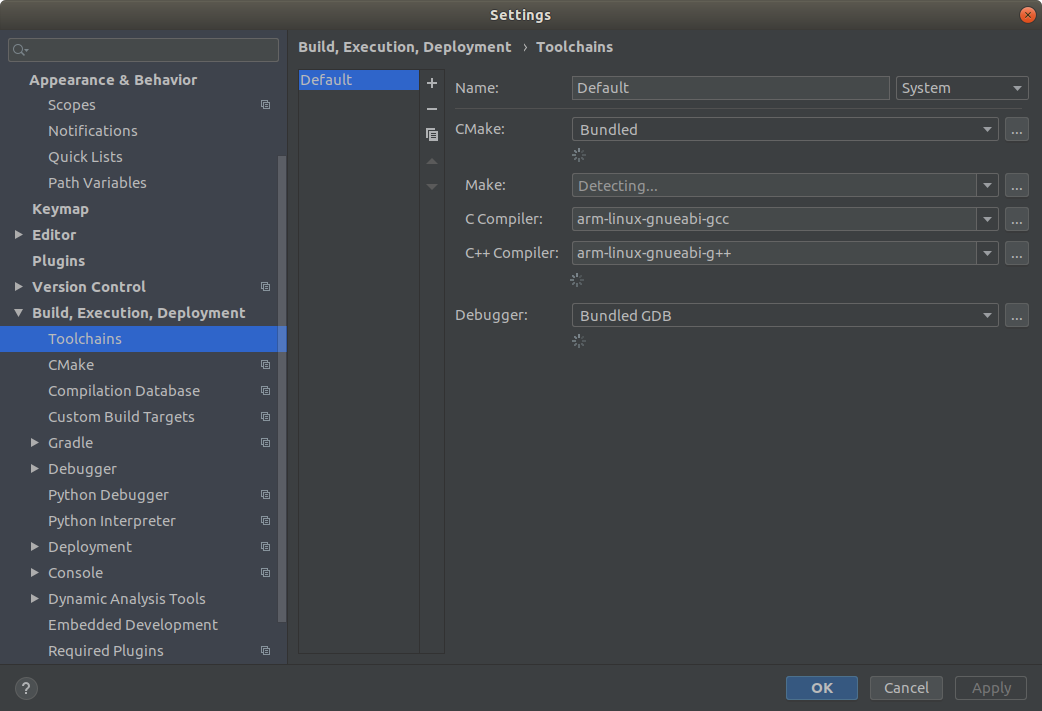
\includegraphics[width=0.8\columnwidth]{Figures/UbuntuCLionConfig}
\caption{CLion Ubuntu Configuration}
\label{fig:UbuntuCLionConfig}
\end{figure}